\documentclass[10pt,xcolor=pdflatex]{beamer}
\usepackage{newcent}
\usepackage[utf8]{inputenc}
\usepackage[czech]{babel}
\usepackage{hyperref}
\usepackage{textpos}
\usepackage{multicol}
\usepackage{tikz}
\usepackage{fancyvrb}
\usepackage{color}
\usepackage{subfig}
\usepackage{geometry}
\usepackage{graphicx}
\usepackage{epstopdf}


\usepackage{todonotes}
\usepackage{listings}

\makeatletter
\g@addto@macro{\UrlBreaks}{\UrlOrds}
\makeatother

\newcommand{\emp}{\lstinline[language={[LaTeX]TeX}, basicstyle=\tt\color{fitdark}]}

\lstdefinelanguage{XML}
{
  basicstyle=\ttfamily\footnotesize,
  morestring=[b]",
  moredelim=[s][\color{red!70!black}]{<}{\ },
  moredelim=[s][\color{red!70!black}]{</}{>},
  moredelim=[l][\color{red!70!black}]{/>},
  moredelim=[l][\color{red!70!black}]{>},
  morecomment=[s]{<?}{?>},
  morecomment=[s]{<!--}{-->},
  commentstyle=\color{black},
  stringstyle=\color{brown!80!black},
  identifierstyle=\color{violet}
}
\lstset{language=Java,
  showspaces=false,
  showtabs=false,
  breaklines=true,
  showstringspaces=false,
  breakatwhitespace=true,
  commentstyle=\color{green!70!black},
  keywordstyle=\color{blue},
  stringstyle=\color{red},
  basicstyle=\ttfamily,
  moredelim=[il][\textcolor{darkgrey}]{\$\$},
  moredelim=[is][\textcolor{darkgrey}]{\%\%}{\%\%}
}

\newcommand{\inlinejava}{\lstinline[language={Java},basicstyle=\ttfamily,keepspaces]}
\newcommand{\inlinejavaEmp}{\color{fitdark}\lstinline[language={Java},basicstyle=\ttfamily,keepspaces]}
\newcommand{\inlinexml}{\lstinline[language={XML},basicstyle=\ttfamily,keepspaces]}
\newcommand{\itmspace}[2]{\item #2 \vspace{#1}}
\newcommand{\tabright}[2]{\dotfill\begin{tabular}[t]{l}{#1}\hspace*{#2}\end{tabular}}
\newcommand{\bcirc}{\tikz\draw[fitblue, fill=fitblue] (0,0) circle (.35ex);}

\newcommand{\radkovani}[1]{\renewcommand{\baselinestretch}{#1}}
\newcommand{\file}[1]{\texttt{#1}}

\epstopdfDeclareGraphicsRule{.gif}{png}{.png}{convert gif:#1 png:\OutputFile}
\AppendGraphicsExtensions{.gif}
\usetheme{FIT}

\def\uv#1{\quotedblbase#1\textquotedblleft}%
\newcommand{\putat}[3]{\begin{picture}(0,0)(0,0)\put(#1,#2){#3}\end{picture}}

%%%%%%%%%%%%%%%%%%%%%%%%%%%%%%%%%%%%%%%%%%%%%%%%%%%%%%%%%%%%%%%%%%
\title[GJA 10]{Android}

\author[]{Jaroslav Dytrych}

\institute[]{Faculty of Information Technology
Brno University of Technology \\
Bo\v{z}et\v{e}chova 1/2. 612 66 Brno - Kr\'alovo Pole\\
dytrych@fit.vut.cz}

\date{28 November 2023}
%\date{\today}
%\date{} % bez data

%%%%%%%%%%%%%%%%%%%%%%%%%%%%%%%%%%%%%%%%%%%%%%%%%%%%%%%%%%%%%%%%%%

\begin{document}

\frame[plain]{\titlepage}

\begin{frame}\frametitle{Contents}
      \begin{itemize}
        \item What is android?
    	\item Android features
        \item Architecture overview
    	\item Environment setup
    	\item Simple applications
    	\item Android database
    	\item Android Java Services
  	  \end{itemize}
\end{frame}


\begin{frame}[fragile]\frametitle{What is Android?}
	\begin{itemize}
		\item Operating system based on Linux and Java
		\item Developed by Google
        \item Dalvik instead of standard JVM (Just-In-Time Compilation)
          \begin{itemize}
            \item replaced by Android Runtime (ART) in Android 5.0
              \begin{itemize}
                \item compatible, but some Dalvik bytecode may not work (ART is less tolerant)
                \item better optimizations (Ahead-of-time (AOT) compilation -- during installation), garbage collection, profiling, \ldots
              \end{itemize}
          \end{itemize}
		\item Android SDK
          \begin{itemize}
        	\item Compiler
              \begin{itemize}
                \item The dx (Dexer) tool converts Java class files into a \texttt{.dex} (ART/Dalvik Executable) file
                \item[] \verb'javac Hello.java'
                \item[] \verb'jar cvf hello.jar Hello.class'
                \item[] \verb'dx --dex --output=helloApp.jar hello.jar'
                \item \texttt{helloApp.jar} will contain \texttt{classes.dex}
                \item Alternatives:
                \item[] \verb'dx --dex --output=classes.dex Hello.class'
                \item[] \verb'dx --dex --output=hello.apk hello.jar'
              \end{itemize}
        	\item Debugger
        	\item Emulator
          \end{itemize}
		\item Google Play (previously Android market)
	\end{itemize}
\begin{tikzpicture}[remember picture,overlay]
    \node[xshift=-0.6cm,yshift=-1.3cm] at (current page.north east){%
    
\includegraphics[width=1cm]{img/pozor}};
\end{tikzpicture}
\end{frame}


\begin{frame}[fragile]\frametitle{File types}
	\begin{itemize}
      \item Application (\texttt{.apk})
        \begin{itemize}
          \item basically improved zip archives with the Java code in a file \texttt{classes.dex}. This file is parsed by the ART/Dalvik JVM and a~cache of the processed \texttt{classes.dex} file is stored in the phone's cache.
          \item created using IDE, Gradle, ant or dx
          \item may contain \textbf{assets} (images, XML files, prefilled databases, \ldots)
        \end{itemize}
      \item \texttt{.odex} (optimized dex) -- pre-processed version of an application's \texttt{classes.dex} that is execution-ready for ART/Dalvik (AOT compiled code)
        \begin{itemize}
          \item only a part of application can be odexed for installing of \texttt{.apk} and \texttt{.odex}
          \item in odexed application the \texttt{classes.dex} is removed from the APK archive and it does not write anything to the cache
          \item Deodexing is basically repackaging of APKs in a certain way, such that they are reassembled into \texttt{classes.dex} files. By doing that, all pieces of an application package are put together back in one place, thus eliminating the worry of a~modified APK conflicting with some separate odexed parts.
        \end{itemize}
	\end{itemize}
\end{frame}

\begin{frame}[fragile]\frametitle{File types}
	\begin{itemize}
	  \item Of Ahead Time (\texttt{.oat})
	    \begin{itemize}
	      \item pre-processed version of an application's \texttt{classes.dex}
	      \item alternative to \texttt{.odex}
	      \item Executable and Linkable Format (ELF)
	    \end{itemize}
      \item Uncompressed DEX (\texttt{.vdex})
        \begin{itemize}
          \item contains the uncompressed DEX code of the APK, with some additional metadata to speed up verification.
          \item Prior Android Oreo (8.0.0) DEX files were embedded in the OAT itself and after Oreo, the transformation performed by dex2oat generates two files.
        \end{itemize}
      \item (\texttt{.art})
        \begin{itemize}
          \item contains ART internal representations of some strings and classes listed in the APK, used to speed application startup.
        \end{itemize}
	\end{itemize}
\end{frame}


\begin{frame}\frametitle{Android features}
	\def\mezera{1em}
	\begin{itemize}
		\item Application ecosystem, allowing to easily add and remove applications and publish new features across the entire system.
		\item Support for all the web technologies, with a browser built on top of the well-established WebKit rendering engine.
		\item Support for hardware accelerated graphics through OpenGL ES (Embedded Systems).
		\item Support for all the common wireless mechanisms: GSM, CDMA, UMTS, LTE, Bluetooth, WiFi.
	\end{itemize}
\end{frame}


\begin{frame}\frametitle{Android versions}
\putat{-30}{-140}{
  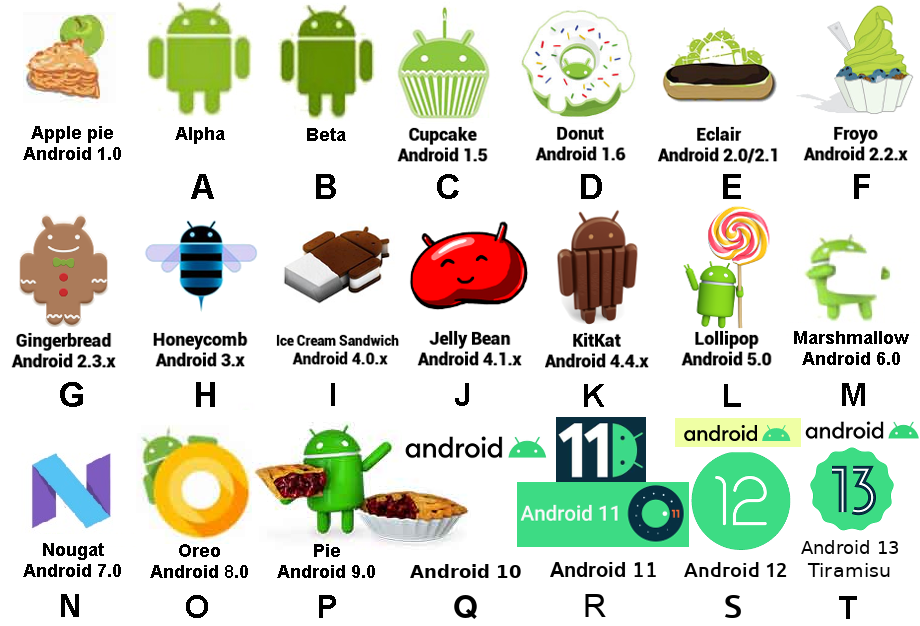
\includegraphics[scale=0.39]{img/android-history7.png}
}
\end{frame}


\begin{frame}\frametitle{Android versions}
\putat{-30}{-140}{
  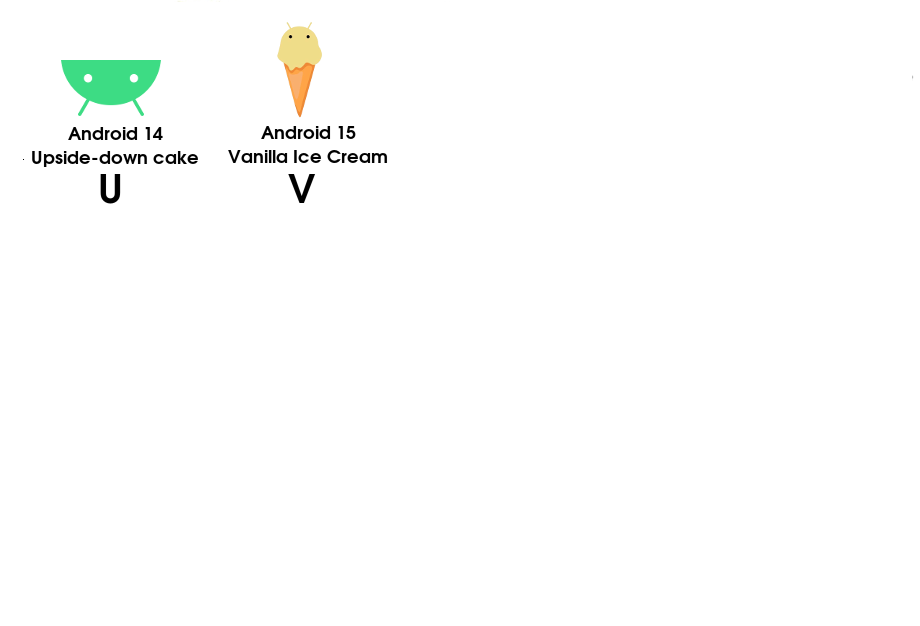
\includegraphics[scale=0.39]{img/android-history2-1.png}
}
\end{frame}


\begin{frame}\frametitle{Android's architecture -- old}
\putat{-16}{-139}{
	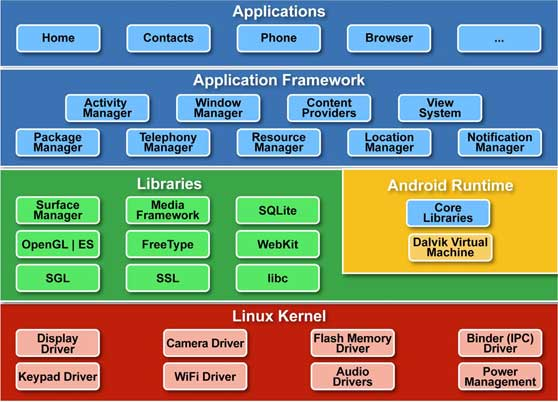
\includegraphics[scale=0.6]{img/pic2.jpg}
}
\end{frame}

\begin{frame}\frametitle{Android's architecture -- new}
\putat{-13}{-139}{
	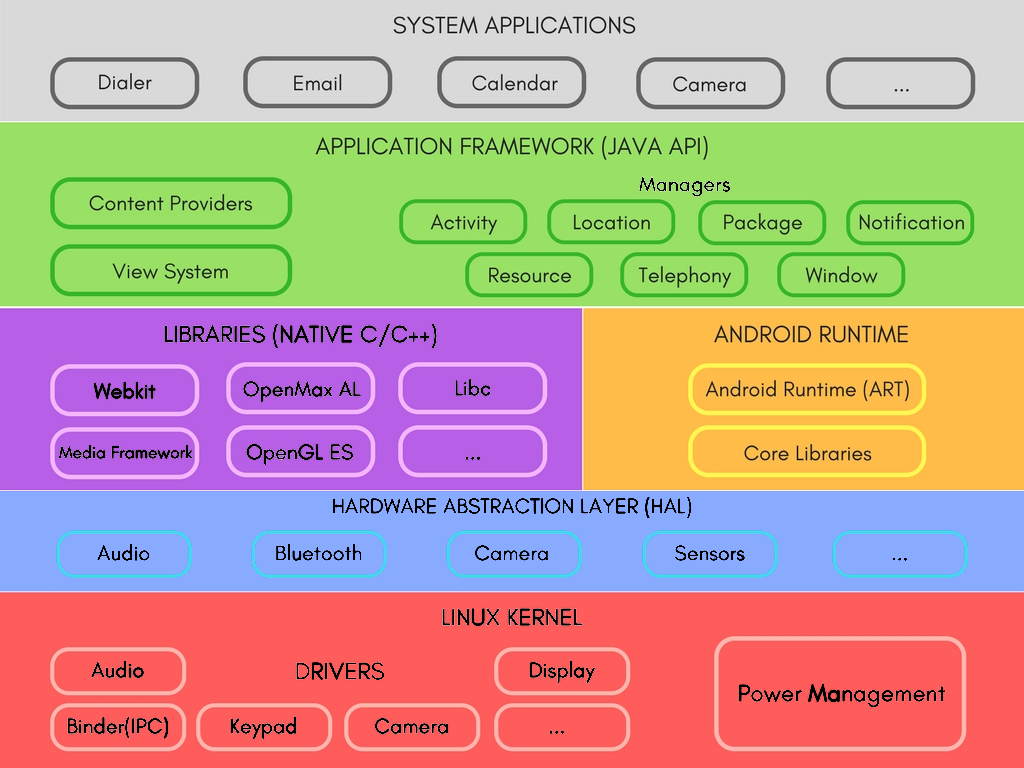
\includegraphics[scale=0.42]{img/android-platform-architecture2.png}
}
\end{frame}

\begin{frame}\frametitle{Android's architecture}
	\begin{itemize}
		\item \emph{Linux kernel} contains all the essential hardware drivers like display, camera, keypad, etc.
        \item \emph{Hardware Abstraction Layer (HAL)} provides abstraction between hardware and rest of the software stack.
        \item \emph{Libraries} includes
          \begin{itemize}
            \item \emph{WebKit} -- a web browser engine,
            \item \emph{SSL} library for the Internet security,
            \item graphic and multimedia libraries \emph{OpenGL ES}, \emph{SGL} (Scalable Graphics Library) and OpenMAX AL (Open Media Acceleration -- Application Layer),
            \item \emph{FreeType} for rendering of fonts,
            \item \emph{Surface Manager} for access to the display subsystem and seamlessly composing of 2D and 3D graphic layers from multiple applications,
            \item \emph{SQLite} for storing of application data (one database per application is expected),
            \item \ldots
          \end{itemize}
	\end{itemize}
\begin{tikzpicture}[remember picture,overlay]
    \node[xshift=-0.6cm,yshift=-1.3cm] at (current page.north east){%
    
\includegraphics[width=1cm]{img/lupa}};
\end{tikzpicture}
\end{frame}


\begin{frame}\frametitle{Android's architecture}
	\begin{itemize}
        \item \emph{Application Framework} is a set of services that collectively form the environment in which Android applications run.
          \begin{itemize}
            \item {\footnotesize \emph{Content Providers} -- allows applications to publish and share data with other applications}.
            \item {\footnotesize \emph{View System} -- is an extensible set of views used to create application user interfaces}.
            \item {\footnotesize \emph{Activity Manager} -- controls all aspects of the application lifecycle and activity stack}.
            \item {\footnotesize \emph{Window Manager} -- is responsible for managing the list of windows, which windows are visible, \ldots}.
            \item {\footnotesize \emph{Package Manager} -- is the system by which applications are able to find out information about other applications currently installed on the device}.
            \item {\footnotesize \emph{Telephony Manager} -- provides information to the application about the telephony services available on the device}.
            \item {\footnotesize \emph{Resource Manager} -- provides access to non-code embedded resources such as strings, color settings and user interface layouts}.
            \item {\footnotesize \emph{Location Manager} -- provides access to the location services allowing an application to receive updates about location changes}.
            \item {\footnotesize \emph{Notifications Manager} -- allows applications to display alerts and notifications to the user}.
          \end{itemize}
	\end{itemize}
\end{frame}


\begin{frame}\frametitle{Security and permissions}
	\begin{itemize}
		\item Unique ID for every application.
          \begin{itemize}
        	\item Applications are separated.
        	\item Sharing is always explicit.
          \end{itemize}
        \item Each application started in own process.
		\item Permissions (for Internet connection, telephone services, camera, \ldots)
          \begin{itemize}
        	\item must be declared in Android manifest.
            \item Different levels of permissions.
            \item User is asked during the installation (up to version 5) or on runtime (From Android 6.0 -- API level 23).
            \item Automatically removed for long-disused applications in newest versions (user can reconfirm on next usage).
          \end{itemize}
	\end{itemize}
\begin{tikzpicture}[remember picture,overlay]
    \node[xshift=-0.6cm,yshift=-1.3cm] at (current page.north east){%
    
\includegraphics[width=1cm]{img/pozor}};
\end{tikzpicture}
\end{frame}


\begin{frame}\frametitle{Android components}
	\begin{itemize}
		\item Activities
          \begin{itemize}
        	\item basically regular applications.
            \item Activity is a screen of user interface (e.g. login activity).
          \end{itemize}
		\item Fragments
          \begin{itemize}
        	\item parts of activities (created from views),
            \item often parts of user interface from 3rd parties.
          \end{itemize}
		\item Views and layout manager
          \begin{itemize}
        	\item buttons, check boxes, text fields, grid layout, linear layout, relative layout, \ldots
          \end{itemize}
 		\item Intents
          \begin{itemize}
        	\item asynchronous messages
            \item between activities
            \item \emph{implicit} (as open the browser) and \emph{explicit} (data transfer).
          \end{itemize}
		\item Services
          \begin{itemize}
        	\item background processes like music players.
          \end{itemize}
		\item Broadcast receivers
          \begin{itemize}
            \item receives intents.
          \end{itemize}
		\item Content providers
          \begin{itemize}
            \item access to the application data and sharing.
          \end{itemize}
	\end{itemize}
\begin{tikzpicture}[remember picture,overlay]
    \node[xshift=-0.6cm,yshift=-1.3cm] at (current page.north east){%
    
\includegraphics[width=1cm]{img/pozor}};
\end{tikzpicture}
\end{frame}



\begin{frame}\frametitle{Environment setup}
	\radkovani{1.2}
	\begin{itemize}
		\item Android SDK
          \begin{itemize}
        	\item Command-line programs
            \item Dalvik/ART executables
          \end{itemize}
		\item Android development tools
          \begin{itemize}
            \item Android Studio (Official IDE for Android based on IntelliJ IDEA)
        	\item Eclipse plugins -- not supported and deprecated (\url{https://dl-ssl.google.com/android/eclipse/})
          \end{itemize}
		\item Android virtual devices
          \begin{itemize}
        	\item Virtual devices manager
          \end{itemize}
        \item ADB (Android Debug Bridge)
          \begin{itemize}
            \item command-line tool that lets you communicate with a device
            \item \emph{client} -- sends commands
            \item \emph{daemon} -- runs commands on a device (background process on each device)
            \item \emph{server} -- manages communication between the client and the daemon (background process on your development machine on port 5037)
          \end{itemize}
	\end{itemize}
    \radkovani{1}
\begin{tikzpicture}[remember picture,overlay]
    \node[xshift=-0.6cm,yshift=-1.3cm] at (current page.north east){%
    
\includegraphics[width=1cm]{img/lupa}};
\end{tikzpicture}
\begin{textblock}{15}(9.9,-0.5)
    {\footnotesize Demo -- SDK manager}
\end{textblock}
\end{frame}


\begin{frame}[fragile]\frametitle{Android debug bridge}
	\begin{itemize}
		\item \texttt{adb install} \verb:<path-to-apk>:
          \begin{itemize}
            \item install an application
          \end{itemize}
        \item \texttt{adb push} \verb:<local>: \verb:<remote>:
          \begin{itemize}
            \item copy a file or directory and its sub-directories to the device
          \end{itemize}
		\item \texttt{adb pull} \verb:<remote>: \verb:<local>:
          \begin{itemize}
            \item copy a file or directory and its sub-directories from the device
          \end{itemize}
		
		\item \texttt{adb forward} \verb:<local-port>: \verb:<remote-port>:
          \begin{itemize}
        	\item e.g. VirtualBox
            \item example: \texttt{adb forward tcp:6100 tcp:7100}
          \end{itemize}
		\item \texttt{adb shell}
          \begin{itemize}
        	\item starts shell in Android environment in the target device
          \end{itemize}
        \item \texttt{adb root}
          \begin{itemize}
            \item Restarts the adbd daemon with root permissions.
          \end{itemize}
        \item \ldots
	\end{itemize}
\end{frame}


%\begin{frame}\frametitle{Project structure -- Eclipse}
%	\begin{itemize}
%		\item \texttt{src}
%		\item \texttt{gen}
%          \begin{itemize}
%        	\item generated Java files
%          \end{itemize}
%		\item \texttt{assets}
%          \begin{itemize}
%        	\item files to be deployed with application (e.g. images)
%          \end{itemize}
%		\item \texttt{libs}
%		\item \texttt{bin}
%          \begin{itemize}
%			\item apk
%            \item dexed classes
%          \end{itemize}
%		\item \texttt{res}
%          \begin{itemize}
%            \item application resources, such as drawable files, layout files and UI string
%            \item often XML files
%          \end{itemize}
%        \item \texttt{AndroidManifest.xml}
%	\end{itemize}
%\begin{tikzpicture}[remember picture,overlay]
%    \node[xshift=-0.6cm,yshift=-1.3cm] at (current page.north east){%
%    
\includegraphics[width=1cm]{img/lupa}};
%\end{tikzpicture}
%\end{frame}


\begin{frame}[fragile]\frametitle{Gradle project structure -- Android Studio}
    \def\twidth{1.5cm}
    \texttt{app}
	\begin{itemize}
      \item \texttt{build} \tabright{(build outputs)}{\twidth}
      \item \texttt{src/main}
        \begin{itemize}
          \item \texttt{assets} \tabright{(images, etc.)}{\twidth}
          \item \texttt{res} \tabright{(application resources)}{\twidth}
          \item \texttt{java} \tabright{(src)}{\twidth}
          \item \texttt{AndroidManifest.xml}
        \end{itemize}
      \item \texttt{app.iml} \tabright{(module IntelliJ IDEA project model)}{\twidth}
      \item \texttt{build.gradle} \tabright{(Gradle script)}{\twidth}
    \end{itemize}
    \texttt{build} \tabright{(build cache, etc.)}{\twidth}\\
    \texttt{gradle}  \tabright{(Gradle wrapper)}{\twidth}\\
    \texttt{AppName.iml} \tabright{(IntelliJ IDEA project model)}{\twidth}\\
    \texttt{build.gradle} \tabright{(Gradle script)}{\twidth}\\
    \texttt{gradlew} \tabright{(Gradle start up script)}{\twidth}\\
    \ldots
\begin{tikzpicture}[remember picture,overlay]
    \node[xshift=-0.6cm,yshift=-1.3cm] at (current page.north east){%
    
\includegraphics[width=1cm]{img/lupa}};
\end{tikzpicture}
\end{frame}

\begin{frame}\frametitle{Assets vs. resources}
	\begin{itemize}
	  \item \emph{Assets} are files to be deployed with application (e.g. images).
	  \item \emph{Resources} are application resources, such as drawable files, layout files and UI string.
	    \begin{itemize}
	        \item Often XML files.
	    \end{itemize}
    \end{itemize}
\end{frame}

\begin{frame}\frametitle{Android manifest}
	\begin{itemize}
		\item File \texttt{AndroidManifest.xml}
        \item unique identifier for the application (Java package name),
          \begin{itemize}
              \item in newest versions moved to \texttt{build.gradle}
          \end{itemize}
        \item the level of the Android API that the application requires -- SDK version (here deprecated -- should be in \texttt{app/build.gradle})
          \begin{itemize}
            \item \texttt{minSdkVersion} -- minimum API Level required for the application to run,
            \item \texttt{targetSdkVersion} -- API Level that the application targets (used for compilation) -- \texttt{targetSdk} in a new version,
            \item \texttt{maxSdkVersion} -- maximum API Level on which the application is designed to run.
          \end{itemize}
        \item used libraries,
		\item permissions setup,
		\item components of the application, which include the activities, services, content providers and broadcast receivers,
        \item entry-point specification,
        \item \ldots
	\end{itemize}
\begin{tikzpicture}[remember picture,overlay]
    \node[xshift=-0.6cm,yshift=-1.3cm] at (current page.north east){%
    
\includegraphics[width=1cm]{img/oko}};
\end{tikzpicture}
\begin{textblock}{15}(9.7,-0.3)
    {\footnotesize Example AndroidImage}
\end{textblock}
\end{frame}


\begin{frame}\frametitle{Android Support Library}
	\begin{itemize}
      \item {\footnotesize When developing apps that support multiple API versions, you may want a~standard way to provide newer features on earlier versions of Android or gracefully fall back to equivalent functionality. Rather than building code to handle earlier versions of the platform, you can leverage these libraries to provide that compatibility layer. In addition, the Support Libraries provide additional convenience classes and features not available in the standard Framework API for easier development and support across more devices.}
    \end{itemize}
\end{frame}


\begin{frame}[fragile]\frametitle{Android Support Library}
	\begin{itemize}
      \item Dependency (Android Studio)
        \begin{itemize}
          \item \texttt{build.gradle} {\footnotesize (Project)}
          \item[] \verb+allprojects {+
          \item[] \verb+  repositories {+
          \item[] \verb+    google()+
          \item[] \verb+    ...+
          \item \texttt{build.gradle} {\footnotesize (Module)}
          \item[] \verb+dependencies {+
          \item[] \verb+  api 'com.android.support:support-v4:28.0.0'+
        \end{itemize}
      \item Installation (Eclipse)
        \begin{enumerate}
          \item {\footnotesize Install Android Support Repository in the SDK manager (Extras).}
          \item {\footnotesize File -- Import.}
          \item {\footnotesize Existing Android Code into Workspace.}
          \item {\footnotesize Browse to the SDK installation directory \texttt{android-sdks/extras/android/support/v7/appcompat}}
          \item {\footnotesize Finish.}
          \item {\footnotesize In the imported library project, expand the \texttt{libs/} folder, right-click each \texttt{.jar} file and select Build Path -- Add to Build Path.}
          \item {\footnotesize Go to the your project properties -- Android category.}
          \item {\footnotesize Add (in the part Library).}
          \item {\footnotesize Select the project and confirm.}
        \end{enumerate}
    \end{itemize}
\end{frame}


\begin{frame}\frametitle{AndroidX}
	\begin{itemize}
	  \item Android Support Library is deprecated.
      \item AndroidX replaces the original support library APIs with packages in the androidx namespace. 
      \item Only the package and Maven artifact names changed; class, method, and field names did not change.
      \item Migration
        \begin{itemize}
            \item Before you migrate, bring your app up to date. It is recommended to update your project to use the final version of the support library: version 28.0.0. This is because AndroidX artifacts with version 1.0.0 are binary equivalent to the Support Library 28.0.0 artifacts.
            \item With Android Studio 3.2 and higher, you can migrate an existing project to AndroidX by selecting Refactor -- Migrate to AndroidX from the menu bar.
        \end{itemize}
    \end{itemize}
\end{frame}


\begin{frame}\frametitle{Activity}
	\begin{itemize}
		\item Activity is a single screen of the user interface of an application.
		\item Activity supports advertising.
		\item When an activity starts a new activity, the latter replaces the former on the screen and is pushed on the back stack which holds the last used activities, so when the user is done with the newer activity, it can easily go back to the previous one
          \begin{itemize}
            \item button Back, gesture or calling of method \texttt{finish()}
          \end{itemize}
	\end{itemize}
\begin{tikzpicture}[remember picture,overlay]
    \node[xshift=-0.6cm,yshift=-1.3cm] at (current page.north east){%
    
\includegraphics[width=1cm]{img/oko}};
\end{tikzpicture}
\end{frame}


\begin{frame}\frametitle{Android activity}
\putat{-28}{-95}{
	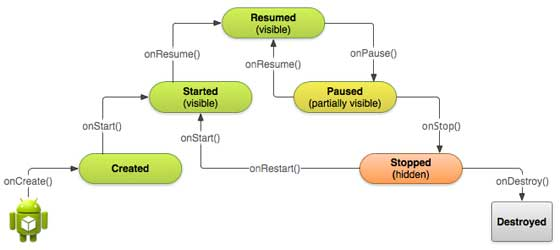
\includegraphics[scale=0.64]{img/pic3.jpg}
}
\begin{tikzpicture}[remember picture,overlay]
    \node[xshift=-0.6cm,yshift=-1.3cm] at (current page.north east){%
    
\includegraphics[width=1cm]{img/pozor}};
\end{tikzpicture}
\end{frame}


\begin{frame}\frametitle{Activity lifecycle}
	\begin{itemize}
        \item Started
          \begin{itemize}
        	\item Created a new Linux process, allocated new memory for the new UI objects, and set up the whole screen (visible).
          \end{itemize}
		\item Running (Resumed)
          \begin{itemize}
        	\item The activity is on the foreground and has focus.
          \end{itemize}
 		\item Paused
          \begin{itemize}
        	\item The activity is still visible on the screen but no longer has focus. It can be destroyed by the system under very heavy memory pressure.
          \end{itemize}
 		\item Stopped
          \begin{itemize}
        	\item The activity is no longer visible on the screen. It can be killed at any time by the system.
            \item It is in the memory for quick restart.
          \end{itemize}
	\end{itemize}
    \medskip
    \begin{itemize}
        \item Each activity extends class \texttt{Activity} with callback methods.
    \end{itemize}
\begin{tikzpicture}[remember picture,overlay]
    \node[xshift=-0.6cm,yshift=-1.3cm] at (current page.north east){%
    
\includegraphics[width=1cm]{img/lupa}};
\end{tikzpicture}
\end{frame}


\begin{frame}\frametitle{Android resources}
	\begin{itemize}
		\item Simple values
          \begin{itemize}
        	\item strings (\texttt{/res/values/strings.xml}),
        	\item constants used in program.
          \end{itemize}
		\item Layouts
          \begin{itemize}
        	\item layout descriptions for activities and fragments.
          \end{itemize}
		\item Styles and themes
          \begin{itemize}
        	\item define appearance (like Holo light with dark action bar).
          \end{itemize}
		\item Animations
          \begin{itemize}
        	\item define animations in XML for the property animation API.
          \end{itemize}
		\item Menus
          \begin{itemize}
        	\item properties of entries for a menu.
          \end{itemize}
	\end{itemize}
\begin{tikzpicture}[remember picture,overlay]
    \node[xshift=-0.6cm,yshift=-1.3cm] at (current page.north east){%
    
\includegraphics[width=1cm]{img/oko}};
\end{tikzpicture}
\end{frame}

\begin{frame}\frametitle{Android resources}
	\begin{itemize}
		\item \texttt{R.java}
          \begin{itemize}
            \item ID's are generated there,
            \item in the XML files we define a names which is mapped into number constants in the generated \texttt{R.java}
            \item[] {\footnotesize \inlinejava{public static final int activity_horizontal_margin=0x7f040000;}}
        	\item constants then can be used to create an objects.
          \end{itemize}
        \item Android Gradle plugin 3.6 and higher includes support for the Maven Publish Gradle plugin, which allows you to publish build artifacts to an Apache Maven repository. Additionally, Android Gradle plugin has made significant performance improvement for annotation processing/KAPT for large projects. This is caused by AGP now generating R class bytecode directly, instead of .java files.
          \begin{itemize}
            \item There is no \texttt{R.java} from Android Studio 3.6.
          \end{itemize}
	\end{itemize}
\begin{tikzpicture}[remember picture,overlay]
    \node[xshift=-0.6cm,yshift=-1.3cm] at (current page.north east){%
    
\includegraphics[width=1cm]{img/oko}};
\end{tikzpicture}
\end{frame}

\begin{frame}[fragile]\frametitle{Resources directory}
	\def\itm[#1]{\item\texttt{#1} -- }
	\begin{itemize}
		\item Resources are stored in \texttt{/res} folder
        \radkovani{1.2}
          \begin{itemize}
        	\itm[anim/]animation definitions,
        	\itm[color/]color definitions,
        	\itm[drawable] subdirectories with images (\texttt{ldpi}, \texttt{mdpi}, \texttt{hdpi}, \texttt{xhdpi}),
        	\itm[layout/]activity layout description,
        	\itm[menu/]menu layout description,
        	\itm[raw/]left untouched,
        	\itm[values/]strings, integers, arrays, etc.,
        	\itm[xml/]arbitrary XML files.
          \end{itemize}
		\radkovani{1}
	\end{itemize}
\end{frame}


\begin{frame}[fragile]\frametitle{Drawable example (1/2) -- custom widget}
	\lstset{language=XML, basicstyle=\footnotesize\ttfamily}
    \begin{lstlisting}
<?xml version="1.0" encoding="UTF-8"?> 
<shape xmlns:android="http://schemas.android.com/apk/res/android" android:shape="rectangle"> 
  <solid android:color="#FF1A47"/>    
  <stroke android:width="3dp"
          android:color="#0FECFF"/> 
  <padding android:left="5dp"
           android:top="5dp"
           android:right="5dp"
           android:bottom="5dp"/> 
  <corners android:bottomRightRadius="7dp"
           android:bottomLeftRadius="7dp" 
           android:topLeftRadius="7dp"
           android:topRightRadius="7dp"/> 
</shape>
    \end{lstlisting}
\end{frame}


\begin{frame}[fragile]\frametitle{Drawable example (2/2) -- custom widget}
	\lstset{language=XML, basicstyle=\footnotesize\ttfamily}
    \begin{lstlisting}
<?xml version="1.0" encoding="UTF-8"?> 
<android:shape 
    xmlns:android="http://schemas.android.com/apk/res/android" 
    android:shape="oval">
  <gradient android:startColor="#31d931" 
            android:endColor="#0da40d" 
            android:angle="270"/>
  <stroke android:width="2dp" android:color="#ffc0c0c0" />
  <size android:height="12dp" android:width="12dp"/>
</android:shape>
    \end{lstlisting}
\end{frame}


\begin{frame}\frametitle{Create first Android application}
	\begin{itemize}
		\item Define Application name, Project name and Package name.
		\item Define SDK and theme of an application
          \begin{itemize}
        	\item minimum SDK version, target SDK version
          \end{itemize}
		\item Configure launcher icon.
		\item Specify type of the main activity.
		\item Specify layout.
		\item Run AVD (Android Virtual Device).
	\end{itemize}
\end{frame}


\begin{frame}\frametitle{User interface controls}
	\begin{itemize}
		\item Control appearance
          \begin{itemize}
        	\item Wrap content
        	\item Match parent (Fill parent)
          \end{itemize}
        \item Define layout/widget with unique ID
          \begin{itemize}
            \item example: \texttt{android:id="@+id/my\_button"}
            \item \texttt{@} --  XML parser should parse and expand the rest of the ID string and identify it as an ID resource.
            \item \texttt{+} -- this is a new resource name that must be created and added to our resources (in the \texttt{R.java} file).
          \end{itemize}
        \item Create an instance of the view object and capture it from the layout
        \item[] {\footnotesize \inlinejava{Button myButton = (Button) findViewById(R.id.my_button);}}
        \ttfamily
        \begin{footnotesize}
        \item Button
		\item CheckBox
		\item Password
		\item RadioButton
		\item ToggleButton
		\item RatingBar
		\item Spinner - drop down menu
		\item ProgressBar
        \item Image
		\item Dialog
        \end{footnotesize}
	\end{itemize}
\begin{tikzpicture}[remember picture,overlay]
    \node[xshift=-0.6cm,yshift=-1.3cm] at (current page.north east){%
    
\includegraphics[width=1cm]{img/naradi}};
\end{tikzpicture}
\begin{textblock}{15}(3.0,-1.4)
    {\footnotesize Examples AndroidCheckBox, AndroidPassword, AndroidRadio}
\end{textblock}
\begin{textblock}{15}(4.7,-0.8)
    {\footnotesize AndroidRatingBar, AndroidSpinner, AndroidProgressBar2}
\end{textblock}
\end{frame}


\begin{frame}[fragile]\frametitle{Dialogs}
	\begin{itemize}
		\item Embedded
          \begin{itemize}
        	\item Prompt
        	\item Alert
            \item[] \texttt{AlertDialog.Builder}
          \end{itemize}
		\item Custom
          \begin{itemize}
        	\item LayoutInflater -- dynamic creation of an instance from XML
        	\item DialogInterface -- defines a dialog-type class
              \begin{itemize}
            	\item \inlinejava{Dialog.class.cast(DialogInterface)}
                \item \texttt{BUTTON\_NEGATIVE, BUTTON\_NEUTRAL, BUTTON\_POSITIVE}
              \end{itemize}
			\item or use \inlinejava{setContentView()}
              \begin{itemize}
            	\item set the activity content to an explicit view (for Dialog)
                \item less dynamic
              \end{itemize}
          \end{itemize}
	\end{itemize}
\begin{tikzpicture}[remember picture,overlay]
    \node[xshift=-0.6cm,yshift=-1.3cm] at (current page.north east){%
    
\includegraphics[width=1cm]{img/naradi}};
\end{tikzpicture}
\begin{textblock}{15}(3.2,2.4)
    {\footnotesize Examples AndroidAlert, AndroidPrompt, AndroidCustomDialog}
\end{textblock}
\end{frame}


\begin{frame}\frametitle{Layout managers}
	\begin{itemize}
		\item \texttt{LinearLayout} -- aligns all children in a single direction, vertically or horizontally
          \begin{itemize}
            \item \texttt{layout\_weight} -- size ratio between multiple views
            \item can be nested
          \end{itemize}
		\item \texttt{RelativeLayout} -- position of each view can be specified as relative to sibling elements (used by designer, easy to break).
		\item \texttt{TableLayout}
		\item \texttt{Listview}
		\item \texttt{GridView}
          \begin{itemize}
        	\item since Android 4.0
          \end{itemize}
		\item \texttt{WebView} -- displays web pages
		\item \texttt{ScrollView}
	\end{itemize}
\begin{tikzpicture}[remember picture,overlay]
    \node[xshift=-0.6cm,yshift=-1.3cm] at (current page.north east){%
    
\includegraphics[width=1cm]{img/kompas}};
\end{tikzpicture}
\begin{textblock}{15}(3.2,0.0)
    {\footnotesize Examples AndroidLinearLayout, AndroidRelativeLayout,}
\end{textblock}
\begin{textblock}{15}(4.9,0.6)
    {\footnotesize AndroidTableLayout, AndroidListView, AndroidGridView}
\end{textblock}
\begin{textblock}{15}(4.9,1.2)
    {\footnotesize AndroidWebView, AndroidScrollView}
\end{textblock}
\end{frame}


\begin{frame}[fragile]\frametitle{Android Intents}
	\begin{itemize}
		\item What are intents?
        \radkovani{1.3}
        \begin{itemize}
        	\footnotesize
        	\item Asynchronous messages which allows Android components to request functionality from other components of the Android system.
        	\item They're signalling, that an event has occurred.
        	\item Sent to system via call {\color{red}\inlinejava{startActivity(Intent)}}.
        	\item Can switch activities of an application.
        	\item Instances of class \inlinejava{android.content.Intent}
        	\item Can be explicit or implicit
              \begin{itemize}
            	\footnotesize
            	\item \emph{Explicit} -- Developer designates the target by its name,
                \item \emph{Implicit} -- There is no explicit target for the Intent. The system will find the best target for the Intent by itself, possibly asking the user what to do if there are several matches (which web browser to use).
              \end{itemize}
			\item Activities, Services and BroadcastReceivers starts using intents.
        \end{itemize}
		\radkovani{1}
	\end{itemize}
\begin{tikzpicture}[remember picture,overlay]
    \node[xshift=-0.6cm,yshift=-1.3cm] at (current page.north east){%
    
\includegraphics[width=1cm]{img/pozor}};
\end{tikzpicture}
\end{frame}


\begin{frame}[fragile]\frametitle{Explicit intents}
	\begin{itemize}
    	\footnotesize
		\item Explicit intents explicitly defines the component which should be called by the Android system, by using the Java class as identifier.
          \begin{itemize}
            \item Associative array of values can be sent in the intent
          \end{itemize}
        \bigskip
        \color{red}
        \item[]
        	\lstset{language=Java, basicstyle=\footnotesize\ttfamily}
            \begin{lstlisting}
Intent i = new Intent(this, ActivityTwo.class);
i.putExtra("Value1", "This is value one for another activity");
            \end{lstlisting}
        \item[]
        	\lstset{language=Java, basicstyle=\footnotesize\ttfamily}
            \begin{lstlisting}
Bundle extras = getIntent().getExtras();
String value1 = extras.getString("Value1");
            \end{lstlisting}
	\end{itemize}
\begin{textblock}{15}(8.8,3.1)
    {\footnotesize Example AndroidExplicitIntent}
\end{textblock}
\end{frame}


\begin{frame}[fragile]\frametitle{Implicit intents}
	\def\mezera{.5em}
	\begin{itemize}
		\item Specify the action which should be performed and optionally data for the action.
		\item If only one handler is registered for an intent, android proceeds with intent directly, otherwise asks user.
          \begin{itemize}
			\item {Like two video players installed \ldots}
          \end{itemize}
		\item[] {{\color{red}\inlinejava{Intent i = new Intent(Intent.ACTION_VIEW, Uri.parse("http://www.fit.vut.cz"));}}}
		\item Serves like global service messages.
	\end{itemize}
\begin{textblock}{15}(8.7,3.9)
    {\footnotesize Example AndroidImplicitIntent}
\end{textblock}
\end{frame}


\begin{frame}\frametitle{Android service}
	\centering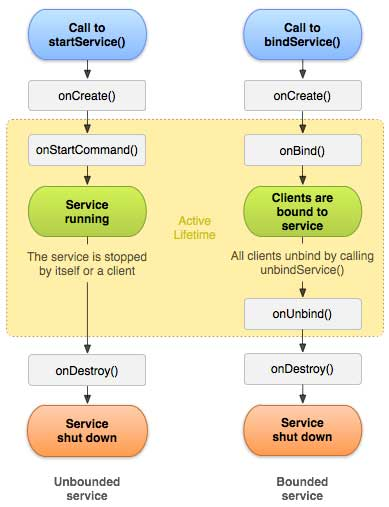
\includegraphics[scale=0.52]{img/pic4.jpg}
\begin{textblock}{15}(4.8,-2.6)
    {\footnotesize interactive}
\end{textblock}
\begin{textblock}{15}(-6.6,-2.6)
    {\footnotesize noninteractive}
\end{textblock}
\begin{tikzpicture}[remember picture,overlay]
    \node[xshift=-0.6cm,yshift=-1.3cm] at (current page.north east){%
    
\includegraphics[width=1cm]{img/lupa}};
\end{tikzpicture}
\end{frame}


\begin{frame}\frametitle{Android service}
  \begin{itemize}
    \item \texttt{onCreate()} -- {\footnotesize executed when the service is first created in order to set up the initial configuration.}
    \item \texttt{onBind()} -- {\footnotesize system invokes this method by calling \texttt{bindService()} when another component wants to bind with the service (such as to perform RPC).}
    \item \texttt{onUnbind()} -- {\footnotesize called when all clients have disconnected from a~particular interface published by the service.}
    \item \texttt{onRebind()} -- {\footnotesize new clients have connected to the service, after it had previously been notified that all had disconnected.}
    \item \texttt{onStartCommand()} -- {\footnotesize executed every time \texttt{startService()} is invoked by another component, like an Activity or a BroadcastReceiver. When this method executes, the service is started and can run in the background indefinitely. If you implement this, it is necessary to stop the service by calling \texttt{stopSelf()} or \texttt{stopService()}.}
    \item \texttt{onDestroy()} -- {\footnotesize the service is no longer used and is being destroyed. Your service should implement this to clean up.}
  \end{itemize}
\end{frame}


\begin{frame}[fragile]\frametitle{Android services}
	\begin{itemize}
		\item Service runs in background without user interaction.
		\item Many predefined services are embedded in system.
		\item Scope resolved in \file{AndroidManifest.xml}
          \begin{itemize}
        	\item in a thread,
            \item in own process.
          \end{itemize}
		\item Services runs with higher priority than activities.
		\item They need to be explicitly declared in manifest.
		\item Communication via Intents.
		\item[] {\inlinejava{OnHandleIntent()}} -- deprecated
        \item[] {\color{red}\inlinejava{OnHandleWork()}}
        \item Activity represents context.
		\item Broadcast receivers reads data from services.
	\end{itemize}
\begin{textblock}{15}(2.0,1.6)
    {\footnotesize Examples AndroidService, AndroidIntentImage, AndroidBoundService}
\end{textblock}
\end{frame}


\begin{frame}[fragile]\frametitle{Broadcast receiver}
	\begin{itemize}
		\item A component which allows to react on custom and system events.
		\item Must be registered
          \begin{itemize}
        	\item either statically in android manifest
            \item or dynamically via \color{red}\inlinejava{Context.registerReceiver()} 
          \end{itemize}
		\item {\color{red}\inlinejava{sendBroadcast(Intent)}} $\to$ {\color{red}\inlinejava{OnReceive(Context, Intent)}}
		\item Intent Filter can be specified.
		\item System broadcasts
          \begin{itemize}
        	\item \verb:BOOT_COMPLETED:
        	\item \verb:CONNECTIVITY_CHANGE:
          \end{itemize}
	\end{itemize}
\end{frame}


\begin{frame}\frametitle{Android Widgets}
	\begin{itemize}
		\item Placed on HomeScreen (e.g. battery indicator).
		\item A Widget runs as a part of the process of its host.
          \begin{itemize}
        	\item This requires that Widgets preserve the permissions of their application.
          \end{itemize}
		\item Uses \texttt{remoteViews} to create user interface.
		\item Interface for a widget is Broadcast receiver.
		\item Steps to create a widget
          \begin{itemize}
        	\item Define layout.
        	\item Create XML -- \texttt{AppWidgetProviderInfo} defined using \texttt{widget\_info.xml}
              \begin{itemize}
                \item Dimensions
                \item Update period
                \item Category (home screen, the keyguard, or both)
              \end{itemize}
        	\item Create a \texttt{BroadcastReceiver} which is used to build the user interface of the Widget.
        	\item Enter the Widget configuration in the \file{AndroidManifest.xml} file.
        	\item Optionally call the activity from the widget.
          \end{itemize}
	\end{itemize}
\begin{textblock}{15}(9.7,0.3)
    {\footnotesize Example AndroidWidget}
\end{textblock}
\begin{tikzpicture}[remember picture,overlay]
    \node[xshift=-0.6cm,yshift=-1.3cm] at (current page.north east){%
    
\includegraphics[width=1cm]{img/oko}};
\end{tikzpicture}
\end{frame}


\begin{frame}\frametitle{Running example AndroidWidget}
	\begin{itemize}
      \item If you have a problem that you have no main activity, in the Android Studio Select menu Run -$>$ Edit Configurations. In the General tab for the app, look for Launch Options and select Nothing instead of Default Activity.
      \item Nothing is visible after installation -- it is necessary to hold finger/pointer on empty space on the home screen and then add the widget.
    \end{itemize}
\end{frame}


\begin{frame}[fragile]\frametitle{Widgets continuation}
	\def\itm[#1]{\item\texttt{#1} -- }
	\begin{itemize}
		\item \texttt{BroadcastReceiver} typically extends \texttt{AppWidgetProvider}.
		\item The \texttt{AppWidgetProvider} class implements the \texttt{onReceive()} method, extracts the required information and calls the following widget lifecycle methods.
		\item Lifecycle
          \begin{itemize}
        	\itm[OnEnabled]when first instance of a widget is added on homescreen.
			\itm[OnDisabled]when the last instance is removed from the homescreen.
			\itm[OnUpdate]everytime a message arrives.
			\itm[OnDeleted]when any instance of a widget is removed from the screen.
          \end{itemize}
	\end{itemize}
\end{frame}


\begin{frame}[fragile]\frametitle{Widget updates}
\begin{itemize}
	\item A Widget gets its data on a periodic timetable.
	  \begin{itemize}
		\item XML configuration updates
		\item \texttt{AlarmManager} service
	  \end{itemize}
    \item Fixed update interval may be specified in XML configuration.
	\item The \texttt{AlarmManager} allows you to be more resource efficient and to have a higher frequency of updates. To use this approach you define a service and schedule this service via the \texttt{AlarmManager} regularly.
\end{itemize}
\begin{tikzpicture}[remember picture,overlay]
    \node[xshift=-0.6cm,yshift=-1.3cm] at (current page.north east){%
    
\includegraphics[width=1cm]{img/oko}};
\end{tikzpicture}
\begin{textblock}{15}(10.0,3.3)
    {\footnotesize Example AlarmActivity}
\end{textblock}
\end{frame}


\begin{frame}[fragile]\frametitle{Android Database system}
\begin{itemize}
	\item Uses open source SQLite database.
	  \begin{itemize}
		\item Supports standard SQL queries.
		\item Requires only 250 kB of memory.
	  \end{itemize}
    \item Supported datatypes
	  \begin{itemize}
		\item \texttt{TEXT} (\texttt{String} in Java),
		\item \texttt{INTEGER} (\texttt{Long} in Java),
		\item \texttt{REAL} (\texttt{Double} in Java).
	  \end{itemize}
    \item Requires accessing the file system.
	  \begin{itemize}
	 	\item Asynchronous processing supported.
	  \end{itemize}
\end{itemize}
\begin{tikzpicture}[remember picture,overlay]
    \node[xshift=-0.6cm,yshift=-1.3cm] at (current page.north east){%
    
\includegraphics[width=1cm]{img/pozor}};
\end{tikzpicture}
\end{frame}


\begin{frame}[fragile]\frametitle{Android SQLite}
\begin{itemize}
  \item No setup needed.
  \item Default database file
  \item[] \texttt{/DATA/APP\_NAME/databases/FILENAME}
    \begin{itemize}
	  \item \texttt{DATA} is the path which the \texttt{Environment.getDataDirectory()} returns.
	  \item \texttt{APP\_NAME} is a name of application.
	  \item \texttt{FILENAME} is a name of a database specified in code.
    \end{itemize}
\end{itemize}
\begin{tikzpicture}[remember picture,overlay]
    \node[xshift=-0.6cm,yshift=-1.3cm] at (current page.north east){%
    
\includegraphics[width=1cm]{img/oko}};
\end{tikzpicture}
\end{frame}


\begin{frame}[fragile]\frametitle{SQLite architecture}
\begin{itemize}
	\item Package \texttt{android.database.sqlite}
	\item \texttt{SQLiteOpenHelper}
	  \begin{itemize}
		\item Manages database updates.
		\item \texttt{onCreate} --  the database is created for the first time (load defaults form assets).
		\item \texttt{onUpdate} -- the database needs to be upgraded. The implementation should use this method to do anything it needs to upgrade to the new schema version.
        \item \texttt{getReadableDatabase()}
		\item \texttt{getWritebleDatabase()}
	  \end{itemize}
    \item Database tables should use \texttt{\_id} as a primary key.
\end{itemize}
\begin{tikzpicture}[remember picture,overlay]
    \node[xshift=-0.6cm,yshift=-1.3cm] at (current page.north east){%
    
\includegraphics[width=1cm]{img/lupa}};
\end{tikzpicture}
\end{frame}

\begin{frame}[fragile]\frametitle{Work with database}
\begin{itemize}
    \item Database installation
      \begin{itemize}
    	\item Check for database existence
        \item[] \texttt{SQLiteDataBase.openDatabase(path, factory, \ldots)}
   		\item If non-existent, copy from Assets.
      \end{itemize}
\end{itemize}
\end{frame}

\begin{frame}[fragile]\frametitle{SQLiteDatabase}
\begin{itemize}
	\item Base type for every database.
	\item Provides methods for working with database
      \begin{itemize}
    	\item \texttt{insert}
		\item \texttt{update}
		\item \texttt{delete}
		\item \texttt{execSQL}
		\item \texttt{rawQuery} -- performs raw SQL query.
		\item \texttt{query} -- structured interface for creating a query.
      \end{itemize}
    \item[]
      \lstset{language=Java, basicstyle=\footnotesize\ttfamily}
      \begin{lstlisting}
Cursor c = getReadableDatabase().rawQuery("select * from todo where _id = ?", new String[] { id });
      \end{lstlisting}
\end{itemize}
\begin{tikzpicture}[remember picture,overlay]
    \node[xshift=-0.6cm,yshift=-1.3cm] at (current page.north east){%
    
\includegraphics[width=1cm]{img/lupa}};
\end{tikzpicture}
\end{frame}


\begin{frame}[fragile]\frametitle{Query parameters}
\begin{itemize}
	\item \texttt{tableName} -- name of the database table.
	\item \texttt{columnNames} -- passing \texttt{null} returns all collumns.
	\item \texttt{whereClause} -- filter, \texttt{null} selects all.
	\item \texttt{selectionArgs} -- \texttt{?}s may be included in the "\texttt{whereClause}"~-- These placeholders will get replaced by the values from the \texttt{selectionArgs} array.
	\item \texttt{groupBy} -- declare how to group rows.
	\item \texttt{having} -- filter, \texttt{null} means no filter.
	\item \texttt{orderBy} -- how to order the results.
	\item[]
      \lstset{language=Java, basicstyle=\footnotesize\ttfamily}
      \begin{lstlisting}
return database.query(DATABASE_TABLE, new String[] {KEY_ROWID, KEY_CATEGORY, KEY_SUMMARY, KEY_DESCRIPTION}, null, null, null, null, null);
      \end{lstlisting}
\end{itemize}
\end{frame}

\begin{frame}[fragile]\frametitle{Cursor}
\begin{itemize}
	\item Query returns cursor object.
	\item Points to one row of returned array.
	\item Has several methods
      \begin{itemize}
    	\item {\color{red}\inlinejava{getCount()}}
        \item {\color{red}\inlinejava{moveToFirst()}}
        \item {\color{red}\inlinejava{moveToNext()}}
        \item {\color{red}\inlinejava{getLong(columnIndex)}}
        \item {\color{red}\inlinejava{getString(columnIndex)}}
        \item {\color{red}\inlinejava{close()}}
        \item \ldots
      \end{itemize}
\end{itemize}
\begin{textblock}{15}(10.3,3.7)
    {\footnotesize Example AndroidSQL}
\end{textblock}
\begin{tikzpicture}[remember picture,overlay]
    \node[xshift=-0.6cm,yshift=-1.3cm] at (current page.north east){%
    
\includegraphics[width=1cm]{img/oko}};
\end{tikzpicture}
\end{frame}


\begin{frame}[fragile]\frametitle{Displaying data}
\begin{itemize}
	\item \texttt{ListView}
      \begin{itemize}
    	\item Adapters -- objects storing collections, that can be displayed.
		\item \texttt{SimpleCursorAdapter} -- defines layout for each row of \texttt{ListView}.
		\item Cursor to view mapping.
      \end{itemize}
    \item Direct usage of \texttt{ListView} is deprecated - use \texttt{ListFragment} instead.
    \item Define arrays
      \begin{itemize}
    	\item An array which contains the column names.
		\item An array which contains the IDs of Views which should be filled with the data.
      \end{itemize}
    \item \texttt{Loader} class
      \begin{itemize}
        \item loads data from a content provider.
      \end{itemize}
\end{itemize}
\end{frame}


\begin{frame}[fragile]\frametitle{Content Provider}
\begin{itemize}
	\item By default, SQLite is private to application.
	\item Sharing can be specified via Content Provider.
	\item Content provider is an application which shares data to other applications, almost allways it is some sort of SQLite database.
	\item Must be specified in manifest
      \begin{itemize}
    	\item \texttt{Android:authorities}
		\item Example -- contacts
      \end{itemize}
    \item Subclasses {\color{red}\inlinejava{android.content.ContentProvider}}
    \item Sharing is implicitly on \texttt{ContentProvider}
      \begin{itemize}
    	\item Can be turned off.
      \end{itemize}
    \item Thread safety
      \begin{itemize}
    	\item Keyword \texttt{synchronized}
      \end{itemize}
\end{itemize}
\begin{textblock}{15}(8.1,1.5)
    {\footnotesize Example AndroidContentProvider}
\end{textblock}
\end{frame}


\begin{frame}[fragile]\frametitle{SQLite full-text search}
\begin{itemize}
	\item {\color{black}\inlinejava{CREATE VIRTUAL TABLE data1 USING fts3(content TEXT);  // inverted index (Apache Lucene)}} 
	\item {\color{black}\inlinejava{CREATE TABLE data2(content TEXT);}} 
    \vspace*{0.5cm}
	\item {\color{black}\inlinejava{SELECT count(*) FROM data1 WHERE content MATCH 'linux';  /* 0.03 seconds */}} 
	\item {\color{black}\inlinejava{SELECT count(*) FROM data2 WHERE content LIKE}} \color{red}\verb|'%linux%'|{\color{black}\inlinejava{; /* 22.5 seconds */}}\color{black}
    \vspace*{0.2cm}
    \item Mapping via rowid/docid (no primary key).
	\item Different query syntax
      \begin{itemize}
   		\item \verb;MATCH;
    	\item Support for wildcards, proximity queries, etc.
		\item Boolean queries.
      \end{itemize}
\end{itemize}
\end{frame}


\begin{frame}[fragile]\frametitle{Android Java Services}
\begin{itemize}
	\item There are lots of services implemented in Java in Android.
	\item They abstract most of the native features to make them available in a consistent way.
	\item Accesible via {\color{black}\inlinejava{Context.getSystemService()}}.
	\item Read the docs for more.
\end{itemize}
\end{frame}

\begin{frame}\frametitle{Android's architecture -- new}
\putat{-13}{-139}{
	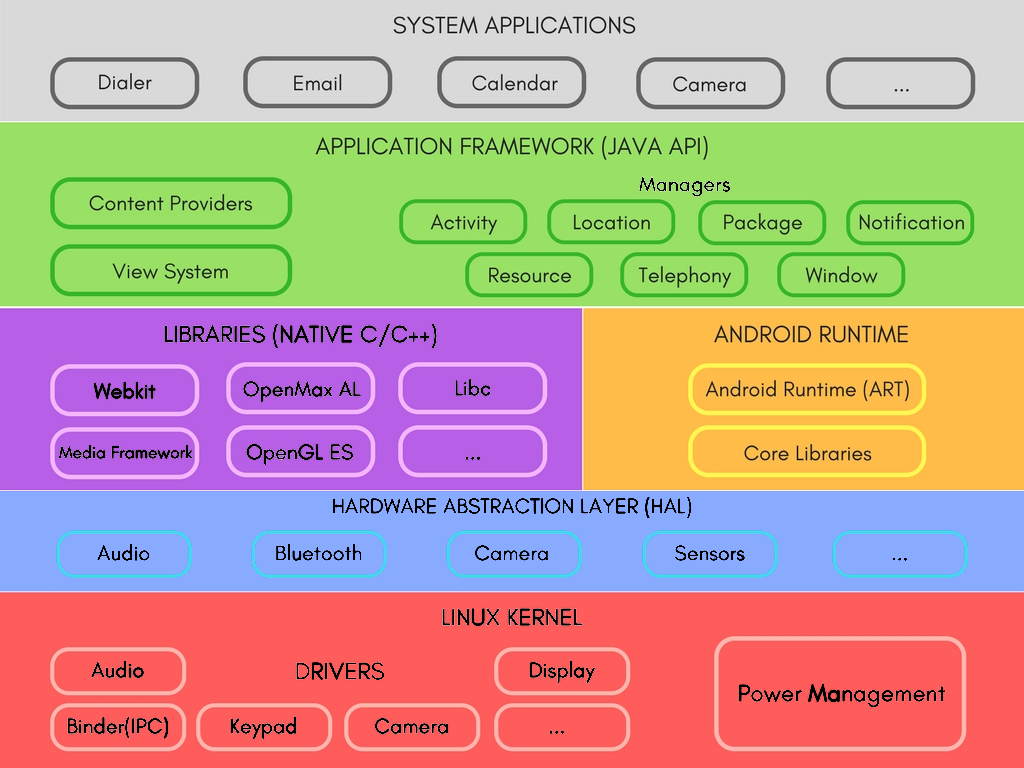
\includegraphics[scale=0.42]{img/android-platform-architecture2.png}
}
\end{frame}

\begin{frame}[fragile]\frametitle{ActivityManager}
\begin{itemize}
    \item ActivityManager manages everything related to Android applications
      \begin{itemize}
    	\item starts activities,
		\item manages their life-cycle,
		\item fetches content from content providers,
		\item handles non-responding applications.
      \end{itemize}
\end{itemize}
\end{frame}


\begin{frame}[fragile]\frametitle{TelephonyManager}
\begin{itemize}
	\item TelephonyManager provides access to information about the telephony services on the device.
    \item \texttt{TelephomyManager.EXTRA\_STATE}
      \begin{itemize}
    	\item \texttt{EXTRA\_STATE\_RINGING}
		\item \texttt{EXTRA\_INCOMING\_NUMBER}
      \end{itemize}
    \item SIM info
	\item Location of the cell
	\item Operator info
\end{itemize}
\end{frame}


\begin{frame}[fragile]\frametitle{PackageManager}
\begin{itemize}
	\item PackageManager is for manipulating already installed packages
	  \begin{itemize}
		\item get list of packages,
		\item get/set permissions,
		\item get details/resources,
		\item install/uninstall package,
		\item check that the application can handle intent of given type.
	  \end{itemize}
\end{itemize}
\end{frame}


\begin{frame}[fragile]\frametitle{AlarmManager}
\begin{itemize}
	\item AlarmManager abstracts timers.
	\item Allows to set one time or repetitive timer.
	\item When a timer expires, the AlarmManager grabs a~wakelock, sends an Intent to the corresponding application and releases the wakelock once the Intent has been handled.
\end{itemize}
\end{frame}


\begin{frame}[fragile]\frametitle{ConnectivityManager}
\begin{itemize}
	\item ConnectivityManager manages network connections.
	  \begin{itemize}
		\item Falls back to other connections when one fails.
		\item Notifies the system when one becomes available/unavailable.
		\item Allows the applications to retrieve various information about connectivity.
	  \end{itemize}
\end{itemize}
\end{frame}


\begin{frame}[fragile]\frametitle{WifiManager}
\begin{itemize}
	\item WifiManager provides an API to manage all aspects of WiFi networks
      \begin{itemize}
    	\item list, modify or delete configured networks,
		\item get information about current WiFi network,
		\item list currently available WiFis,
		\item send intents on changes.
      \end{itemize}
\end{itemize}
\end{frame}


\begin{frame}[fragile]\frametitle{NotificationManager}
\begin{itemize}
	\item NotificationManager notifies the user of events that happen. This is how you tell the user that something has happened in the background.
	\item Notifications can take different forms:
      \begin{itemize}
    	\item A persistent icon that goes in the status bar and is accessible through the launcher,
    	\item Turning on or flashing LEDs on the device,
    	\item Alerting the user by flashing the backlight, playing a sound, or vibrating.
      \end{itemize}
\end{itemize}
\end{frame}



\begin{frame}[fragile]\frametitle{Other managers}
\begin{itemize}
	\item PowerManager
	\item LocationManager
    \item ClipboardManager
    \item \ldots
\end{itemize}
\begin{tikzpicture}[remember picture,overlay]
    \node[xshift=-0.6cm,yshift=-1.3cm] at (current page.north east){%
    
\includegraphics[width=1cm]{img/kompas}};
\end{tikzpicture}
\end{frame}


\begin{frame}[fragile]\frametitle{System server}
\begin{itemize}
	\item Starts all system services and managers.
	\item Runs services as:
	  \begin{itemize}
	      \item Lights Service,
	      \item Vibrator Service,
	      \item Sensor Service,
	      \item \ldots
	  \end{itemize}
\end{itemize}
\begin{tikzpicture}[remember picture,overlay]
    \node[xshift=-0.6cm,yshift=-1.3cm] at (current page.north east){%
    
\includegraphics[width=1cm]{img/lupa}};
\end{tikzpicture}
\end{frame}


\begin{frame}[fragile]\frametitle{References 1/4}
\begin{itemize}
	\item Vogella: Getting started with Android development
      \begin{itemize}
    	\begin{footnotesize}
    	\item \url{http://www.vogella.com/articles/Android/article.html}
        \end{footnotesize}
      \end{itemize}
    \item Mkyong: Android Tutorial
      \begin{itemize}
    	\begin{footnotesize}
    	\item \url{http://www.mkyong.com/tutorials/android-tutorial/}
        \end{footnotesize}
      \end{itemize}
    \item Tutorials Point: Android Tutorial
      \begin{itemize}
    	\begin{footnotesize}
    	\item \url{https://www.tutorialspoint.com/android/index.htm}
        \end{footnotesize}
      \end{itemize}
    \item Learn Android Development
      \begin{itemize}
        \item \url{https://www.studytonight.com/android/}
      \end{itemize}
    \item Documentation
      \begin{itemize}
        \item \url{https://developer.android.com}
      \end{itemize}
\end{itemize}
\end{frame}

\begin{frame}[fragile]\frametitle{References 2/4}
\begin{itemize}
    \item Others
      \begin{itemize}
        \footnotesize
        \item \url{https://www.businessinsider.com/how-android-was-created-2015-3}
        \item \url{https://www.digitaltrends.com/mobile/android-version-history/}
        \item \url{https://www.techuntold.com/sequence-behind-android-os-names/}
        \item \url{http://www.techotopia.com/index.php/An_Overview_of_the_Android_Architecture}
        \item \url{https://www.boldare.com/blog/differences-between-class-and-dex-files-in-java-android/}
        \item \url{http://darutk-oboegaki.blogspot.cz/2011/03/usage-of-dx-dex-dx-dex.html}
        \item \url{http://stackoverflow.com/questions/9593527/what-are-odex-files-in-android}
        \item \url{http://www.addictivetips.com/mobile/what-is-odex-and-deodex-in-android-complete-guide/}
        \item \url{https://web.archive.org/web/20171108061932/http://www.limbaniandroid.com/2014/04/how-to-display-datepickerdialog-in.html}
        \item \url{https://stackoverflow.com/questions/45373007/progressdialog-is-deprecated-what-is-the-alternate-one-to-use}
        \normalsize
      \end{itemize}
\end{itemize}
\end{frame}

\begin{frame}[fragile]\frametitle{References 3/4}
\begin{itemize}
    \item Others
      \begin{itemize}
        \footnotesize
        \item \url{https://lief.quarkslab.com/doc/latest/tutorials/10_android_formats.html}
        \item \url{https://www.geeksforgeeks.org/how-to-create-a-basic-widget-of-an-android-app/}
        \item \url{https://www.slideshare.net/opersys/understanding-the-android-system-server}
        \item{\url{https://stackoverflow.com/questions/62138507/intentservice-is-deprecated-how-do-i-replace-it-with-jobintentservice}}
        \item{\url{https://medium.com/mindorks/android-jobintentservice-for-background-task-e77bfa21fffa}}
        \item \url{https://android-developers.googleblog.com/2020/02/android-studio-36.html}
        \item \url{https://stackoverflow.com/questions/43923996/adb-root-is-not-working-on-emulator-cannot-run-as-root-in-production-builds}
        \item \url{https://jfrog.com/blog/into-the-sunset-bintray-jcenter-gocenter-and-chartcenter/}
        \item \url{https://stackoverflow.com/questions/49612534/share-a-resource-image-with-intents}
        \normalsize
      \end{itemize}
\end{itemize}
\end{frame}

\begin{frame}[fragile]\frametitle{References 4/4}
\begin{itemize}
    \item Others
      \begin{itemize}
        \footnotesize
        \item \url{https://stackoverflow.com/questions/61023968/what-do-i-use-now-that-handler-is-deprecated}
        \item \url{https://stackoverflow.com/questions/58767733/android-asynctask-api-deprecating-in-android-11-what-are-the-alternatives}
        \item \url{https://developer.android.com/training/scheduling/alarms}
        \item \url{https://stackoverflow.com/questions/68473542/mediasessioncompattargeting-s-version-31-and-above-requires-that-one-of-flag}
        \item \url{https://www.linuxtopia.org/online_books/android/devguide/guide/topics/appwidgets/index.html}
        \item \url{https://www.sqlite.org/fts3.html}
        \normalsize
      \end{itemize}
\end{itemize}
\end{frame}


\bluepage{Thank you for your attention!}



\end{document}
